\documentclass[t,xcolor={svgnames,table}]{beamer}

\mode<presentation>
\usetheme{Warsaw}
\useoutertheme{infolines} 

\usepackage{lmodern}
\usepackage{amsmath}
\usepackage{amsfonts}
\usepackage{bbm}
\usepackage{bm}
\usepackage{nicefrac}
\usepackage{color}
\usepackage{multirow}
\usepackage{multicol}
\usepackage{adjustbox}
\usepackage{tikz}
\usepackage{tikz-dependency}
\usepackage{tikz-qtree}
\usepackage{pgfplots,pgfplotstable}
\usepackage{pgf}
\usepackage{collcell}
\usepackage{booktabs}
\usepackage{soul}

\definecolor{yellow}{rgb}{0.89, 0.61, 0.06}
\definecolor{green}{rgb}{0.0, 0.5, 0.0}
\definecolor{red}{rgb}{0.7, 0.11, 0.11}

% Outline slides
\AtBeginSection[]
{\begin{frame} \frametitle{Outline} \tableofcontents[currentsection,currentsubsection] \end{frame}}

\begin{document}


\title[]{The Language of Legal and Illegal Activity \\ on the Darknet}
\author[Daniel Hershcovich]{Leshem Choshen, Dan Eldad, \textbf{Daniel Hershcovich}, \\
Elior Sulem and Omri Abend }
\date[]{ACL 2019 \\
	\hspace{0.5cm}

\includegraphics[width=.5\textwidth]{huji_banner.png}

\includegraphics[width=.1\textwidth]{huji_logo.jpg}}

\begin{frame}
\titlepage
\end{frame}

\section*{Introduction}

{\usebackgroundtemplate{
	\vbox to \paperheight{\vfil\hbox to \paperwidth{\hfil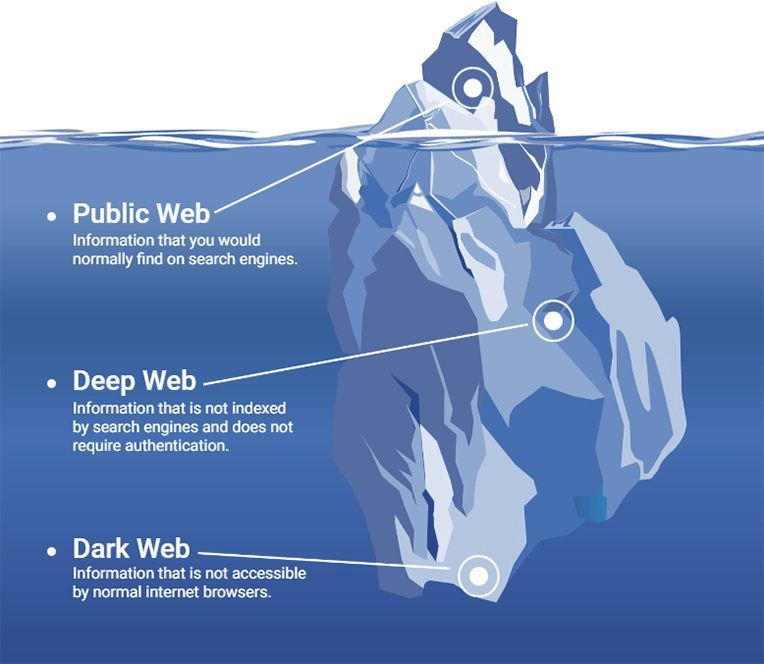
\includegraphics[width=.92\paperwidth]{DarkNet}\hfil}}	
	}%
\begin{frame}
	What is the Dark Web?
	% TODO: examples
\end{frame}
}

\begin{frame}
	\frametitle{Darknet}
	
	Used interchangeably in this work:
	\vfill
	
	\begin{minipage}{.6\pagewidth}
	\begin{itemize}\setlength\itemsep{1em}
	\item \textbf{Dark Web}
	\item \textbf{Darknet}
	\item \textbf{Tor} network (Tor: an encrypted browser)
	\item \textbf{Onion} network (.onion top-level domain)
	\end{itemize}
	\end{minipage}
	\begin{minipage}{.3\pagewidth}
	
\includegraphics[width=.3\pagewidth]{Tor.png}
	\end{minipage}
	\vfill
	
	Hosts: \textbf{onion services} (hidden services).
\end{frame}

\begin{frame}
	\frametitle{Darknet Markets}
	
	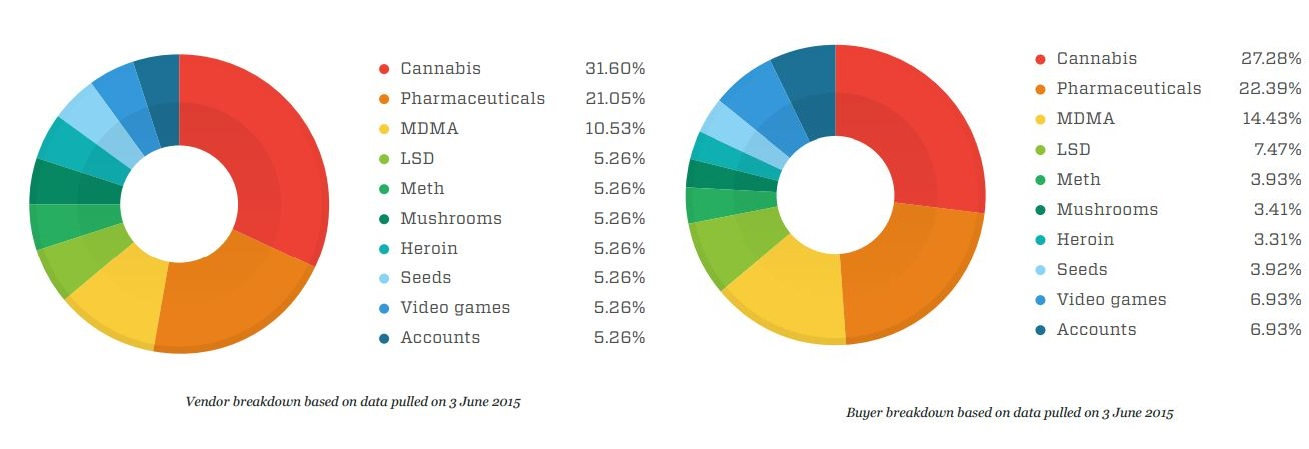
\includegraphics[trim={0 2cm 16cm 1cm},clip,width=\pagewidth]{DeepWeb-Black-markets-vendors-buyers.jpg}\footnote{Paganini (2015). "The Deep Web and Its Darknets".}
\end{frame}

\section{Data: Darknet \& eBay}

\begin{frame}
	\frametitle{DUTA-10K}
	\begin{itemize}\setlength\itemsep{1em}
		\item DUTA-10K, illegal vs. legal drugs \cite{AlNabki19}.
		\item Contains 10367 websites (Hidden Services).
		\item 20\% are illegal and 48\% are legal (32\% unavailable).
		\item Illegal drugs are 23\% of illegal websites.
	\end{itemize}
\end{frame}

\begin{frame}
	\frametitle{Control Data: eBay}
	Manually acquired eBay products of drugs weed etc. % change "etc." to actual list
	\vfill
	
	\begin{center}
	
\includegraphics[width=.5\textwidth]{ebay.png}
	\end{center}
\end{frame}

\begin{frame}
	\frametitle{Data}
	\begin{center}
	\def\arraystretch{2}
	\begin{tabular}{c|cc}
	& Public Web & Dark Web \\ 
	\hline
	Legal & \textbf{\color{yellow} eBay} & \textbf{\color{green} Legal Onion} \\
	Illegal & & \textbf{\color{red} Illegal Onion}
	\end{tabular}
	\end{center}
\end{frame}

\begin{frame}
	\frametitle{Cleaning}
	% TODO
\end{frame}

\section{Domain Differences: Vocabulary \& Named Entities}

\begin{frame}
	\frametitle{Vocabulary}
	Jensen-Shannon divergence and variational distance between word frequencies.
	Self distances are small while pair distances in Legal-Illegal-eBay are high.
	
	Legal and Illegal should be considered different domains, despite being both DarkNet material.
	\begin{figure}
		\centering
		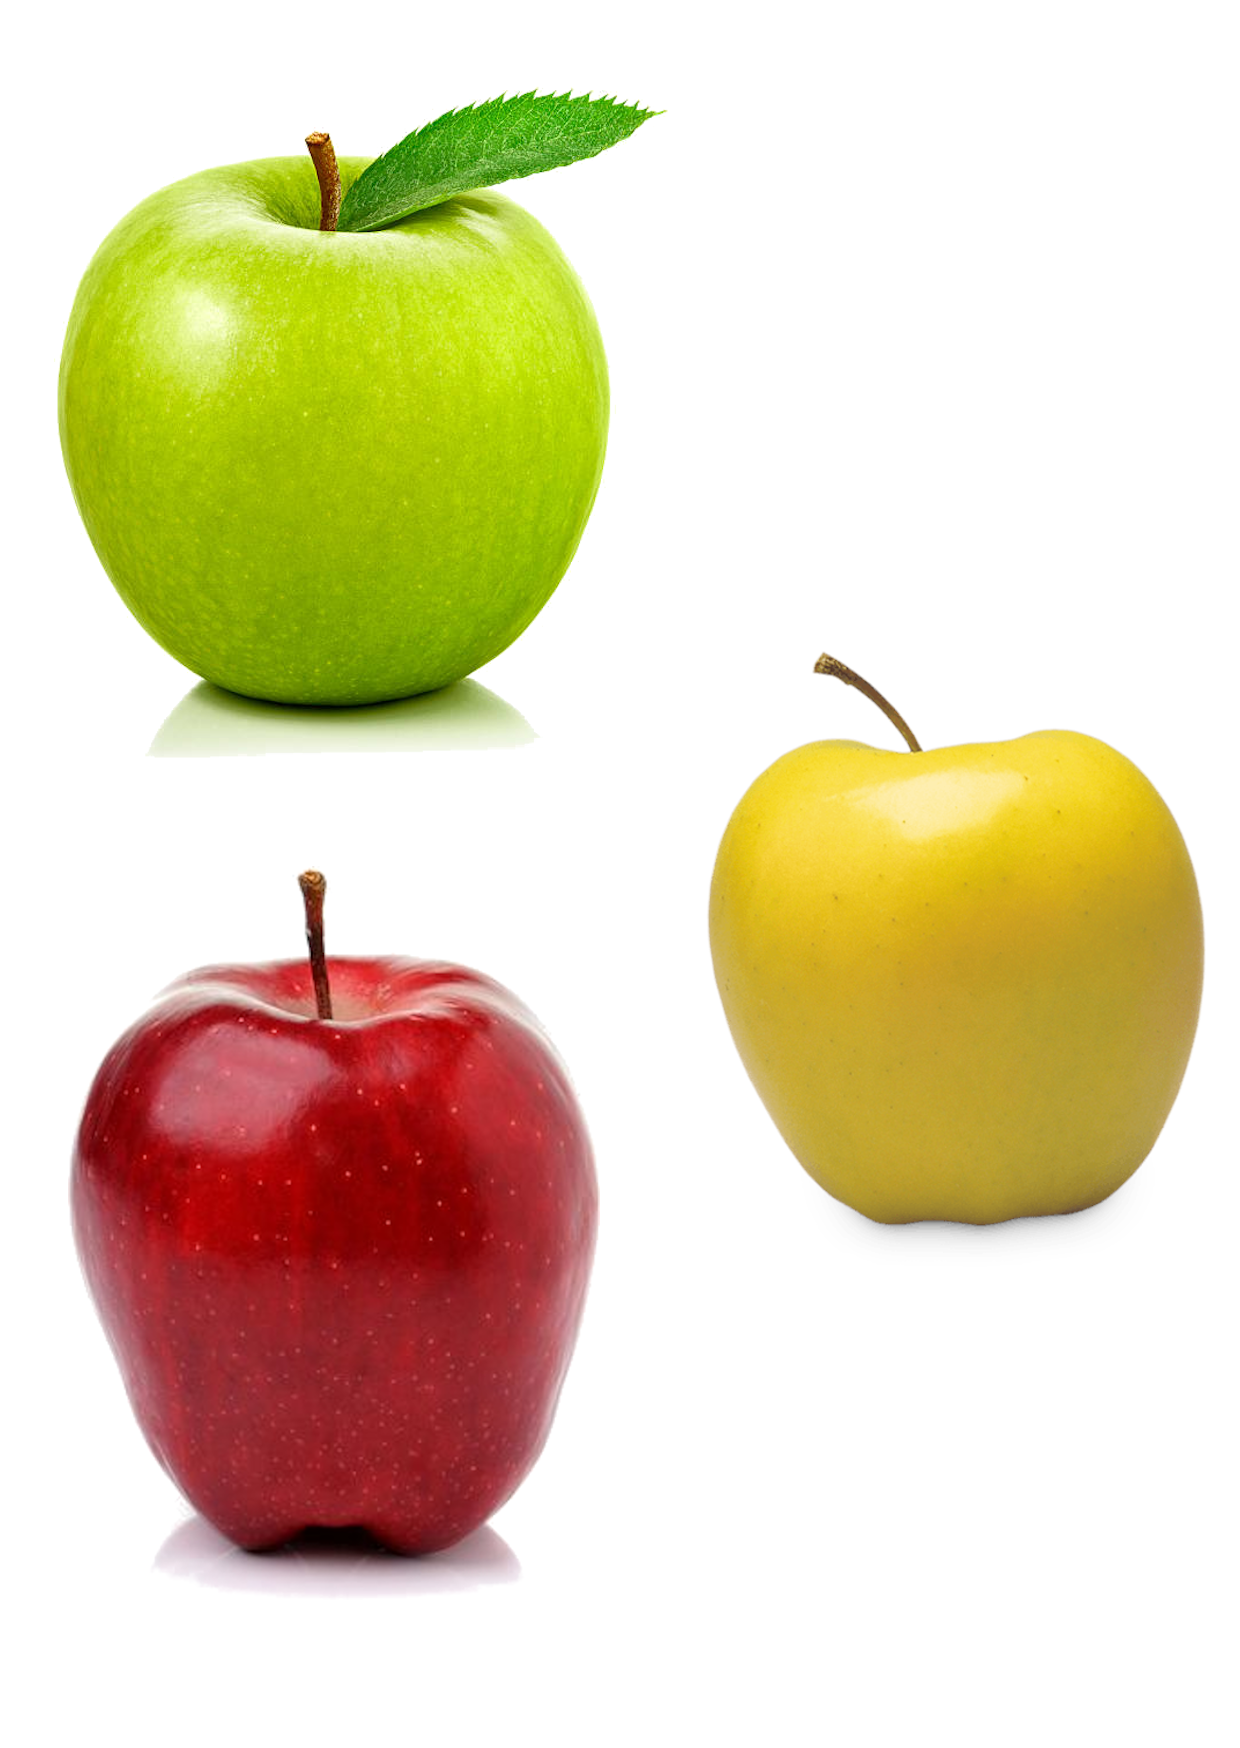
\includegraphics[width=0.3\textwidth]{3different.png}
	\end{figure}
	% TODO: some quantitative results

\end{frame}

\begin{frame}
	\frametitle{Named Entities and Wikification}
	% TODO
\end{frame}

\section{Classification: Legal \& Illegal Drugs, eBay}

\begin{frame}
	\frametitle{Classes}
	We identified three domains:
	\begin{center}
	\{ \textbf{\color{yellow} eBay}, \textbf{\color{green} Legal Onion}, \textbf{\color{red} Illegal Onion} \}
	\end{center}
	\vfill
	
	What are the linguistic features distinguishing them?
	\vfill
	
	\begin{center}
	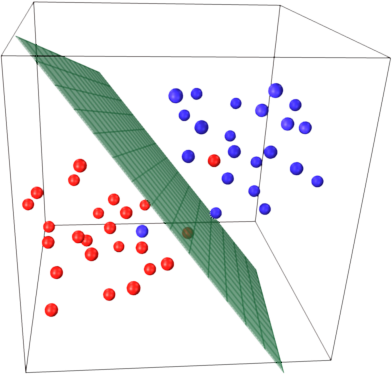
\includegraphics[width=.3\textwidth]{svm.png}
	\end{center}
\end{frame}

\begin{frame}
	\frametitle{Classifiers}
	
	\begin{minipage}{.7\textwidth}
	\begin{itemize}\setlength\itemsep{1em}
		\item NB: Naive Bayes
		\item SVM: Support Vector Machine
		\item BoE: sum/average GloVe + MLP
		\item seq2vec: BiLSTM + MLP
		\item attention: ELMo + BCN (self-attention)
	\end{itemize}
	\end{minipage}
	\begin{minipage}{.29\textwidth}
	\centering
	\hspace{-2cm}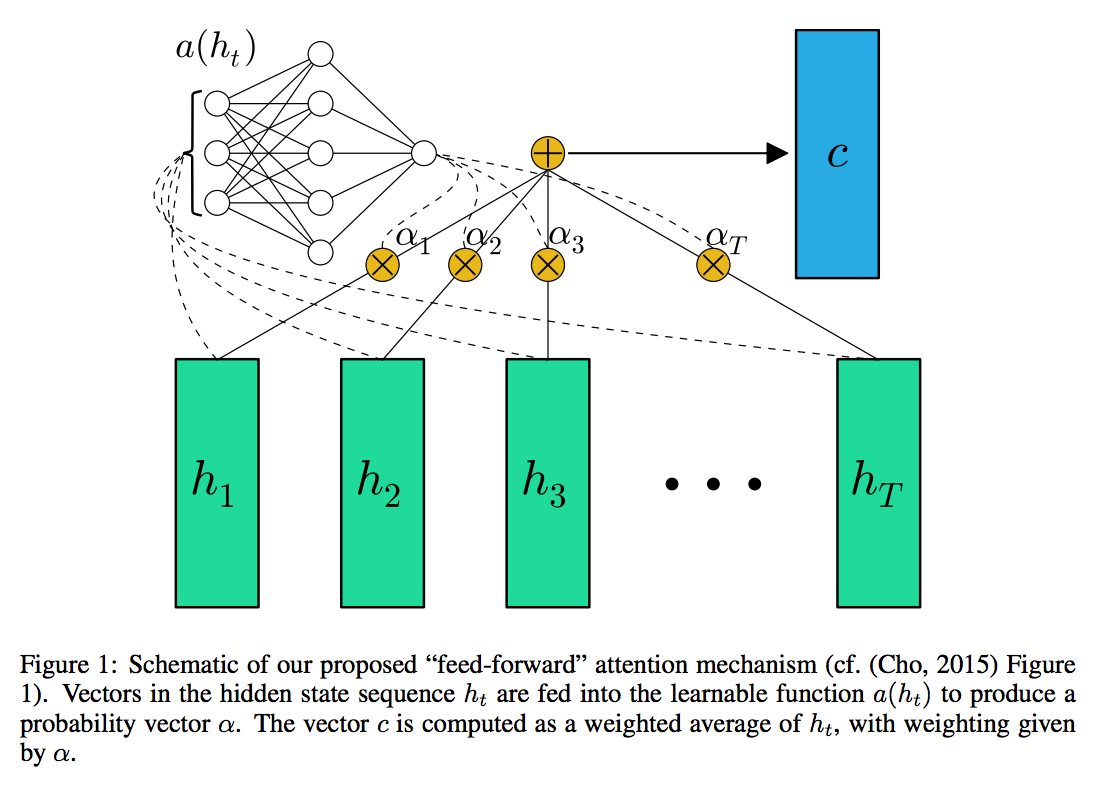
\includegraphics[trim={3cm 3cm 3cm 0},clip,width=1.5\textwidth]{FeedForwardAttention.png}
	
	
\includegraphics[width=.7\textwidth]{elmo.jpg}
	\end{minipage}
\end{frame}

\begin{frame}
	\frametitle{Manipulations}
	
	\begin{itemize}\setlength\itemsep{1em}
	    \item Full original text
	\end{itemize}
	\vfill
	
	\begin{minipage}{.35\textwidth}
	\begin{itemize}\setlength\itemsep{1em}
		\item Drop \textbf{content} words
		\item Drop \textbf{function} words
	\end{itemize}
	\end{minipage}
	\begin{minipage}{.59\textwidth}
	\begin{itemize}\setlength\itemsep{1em}
		\item Replace \textbf{content} words with their POS
		\item Replace \textbf{function} words with their POS
	\end{itemize}
	\end{minipage}
	\vfill
	
    \[\{\textsc{adj, adv, noun, propn, verb, x, num}\}\]
	\vfill
	\pause
	
	{\color{green}
	\setlength{\tabcolsep}{2.3pt}
	\begin{tabular}{ccccccccccc}
	Generic&Viagra&(&Oral&Jelly&)&is&used&for&Erectile&Dysfunction\\
	\small\textsc{propn} & \small\textsc{propn} &(& \small\textsc{propn} & \small\textsc{propn} &)& \small\textsc{verb} & \small\textsc{verb} & for & \small\textsc{propn} & \small\textsc{propn}
	\end{tabular}}
	\vfill
	\pause
	
	{\color{red}
	\setlength{\tabcolsep}{9.5pt}
	\begin{tabular}{ccccccc}
	Welcome&to&SnowKings&Good&Quality&Cocaine&!\\
	\small\textsc{verb} & to & \small\textsc{propn} & \small\textsc{propn} & \small\textsc{propn} & \small\textsc{propn} & !
	\end{tabular}}
\end{frame}

\begin{frame}
	\frametitle{legal DarkNet vs. eBay}
\end{frame}

\begin{frame}
	\frametitle{legal Drugs vs. illegal}
\end{frame}

\section{Cross-Domain Classification: Legal \& Illegal Forums}

\begin{frame}
	\frametitle{cross domain illegality}
	Forum: multi-topic\footnote{\textit{We assign Forum label to the multitopic forums unless the whole forum is related to
a single topic. e.g. a hacking forum was assigned
to Hacking class instead of Forum.}} \cite{AlNabki17}
\end{frame}

\section*{}

\begin{frame}
\frametitle{Conclusion}
\end{frame}

\begin{frame}[allowframebreaks]
\frametitle{References}
\bibliographystyle{apalike}
\tiny\bibliography{acl2019}
\end{frame}

\end{document}
